% Related Works wording supplied by the author; citations mapped to existing bibliography keys.
\section{Related Works}

% INTEGRATION-BEGIN
\begin{figure*}[!t]
\centering
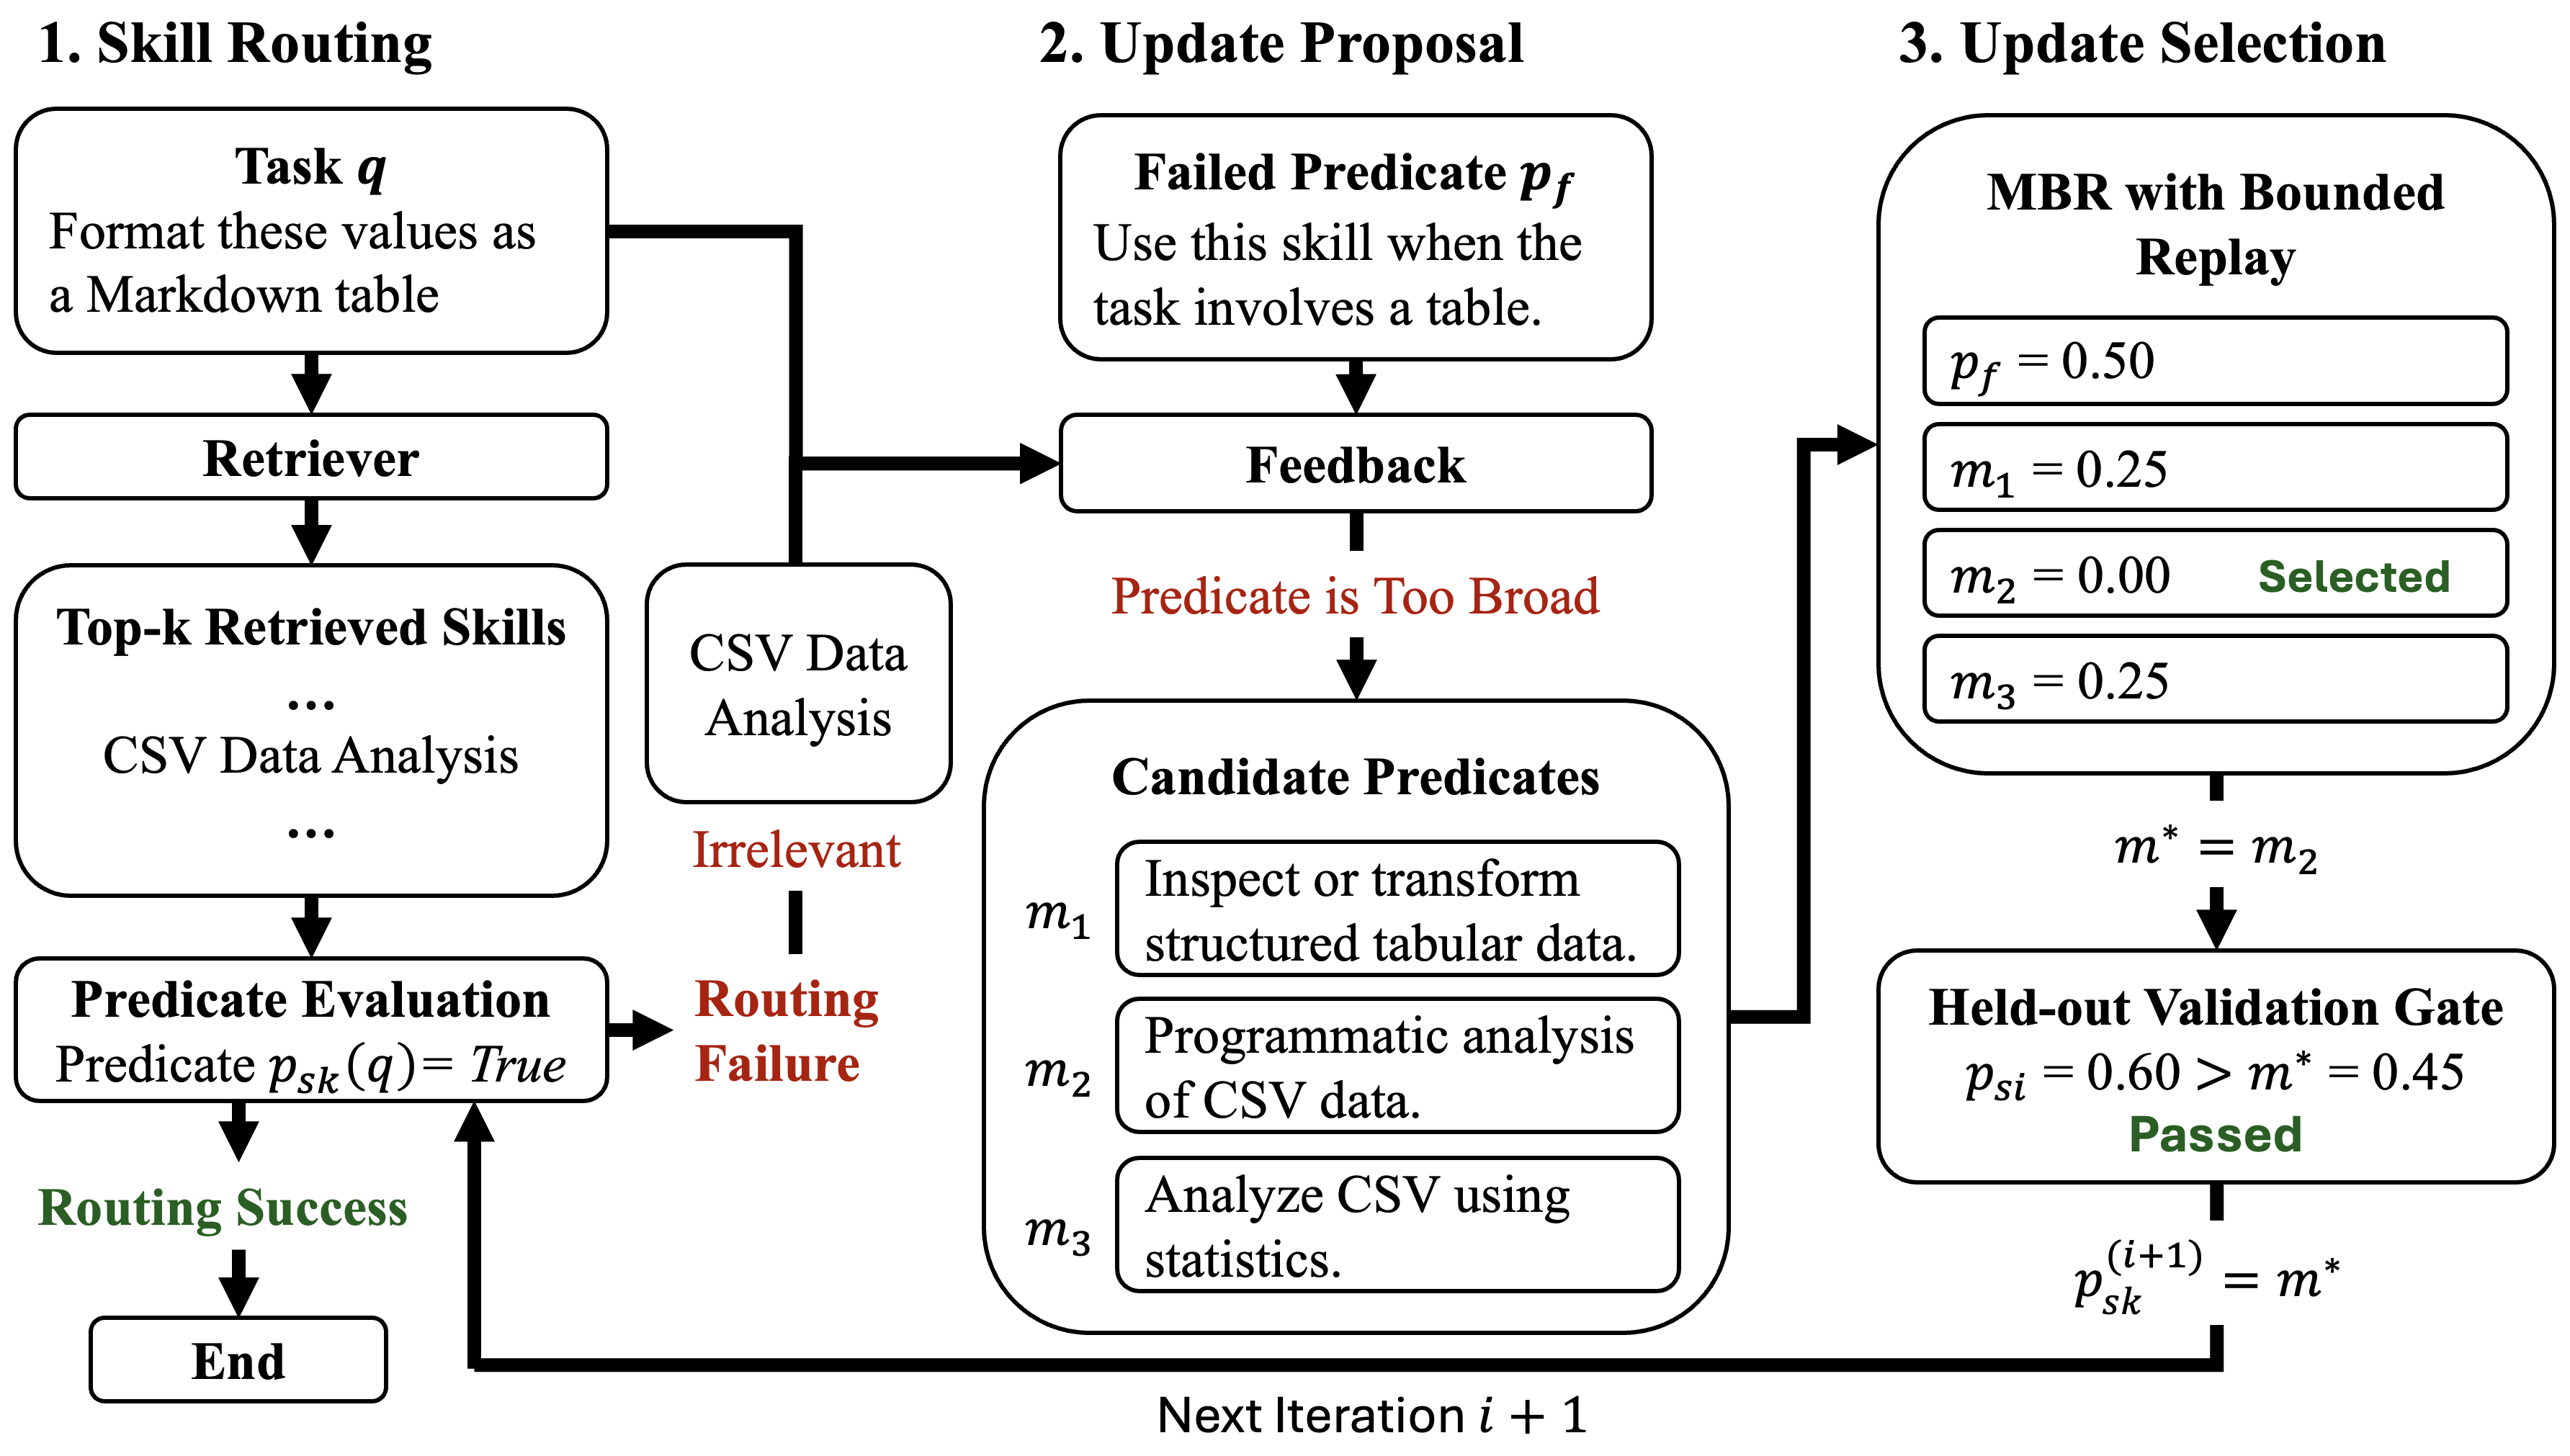
\includegraphics[width=\textwidth]{figs/method_figure.png}
\caption{RouterBSI’s bayes self-improvement algorithm of predicate $p_{sk}$ for the skill $\mathrm{s}_{\mathrm{k}}$ in top k. Routing failures drive revisions selected which are selected based on their bounded replay error using Minimum Bayes Risk (MBR). Selected candidate is discarded by the held-out validation gate if its validation error is higher or equal to the initial predicate $\mathrm{p}_{\mathrm{si}}$.}
\label{fig:routerbsi-overview}
\end{figure*}
% INTEGRATION-END

\subsection{Non-Parametric Routing Optimization}
Non-parametric routing optimization updates external routing state from task feedback while keeping model weights fixed. Experience-based methods revise memories and procedures, but revisions can undo earlier improvements \citep{wang2025agentworkflowmemory,ouyang2026reasoningbank,guo2024dsagent}. Structural methods evolve skill relationships, but graph expansions can introduce many irrelevant skills, reducing precision or exceeding context limits \citep{zhang-etal-2025-toolexpnet,bai2026skilldag}. Gated updates limit regressions through surrogate objectives or rollback criteria but don’t directly minimizing routing error on seen tasks \citep{pmlr-v306-mi26d,shi2026programmatic}. Similar to our approach, JTPRO evaluates candidates on sampled training minibatches and held-out validation but does not provide bounded experience management for online adaptation \citep{ghoshal-etal-2026-jtpro}. Retaining earlier routing corrections while bounding experience and evaluation costs remains a challenge. RouterBSI ensures non-increasing empirical error on the retained set while bounding replay evaluation costs. A held-out gate additionally rejects updates that regress validation performance below the cold-start performance.

\subsection{Parametric Routing Optimization}
Parametric routing optimization updates model weights using supervision, preferences, or execution feedback. Learned retrievers and rerankers score relevance or utility of skill for task \citep{qin2024toolllm,zheng2026skillrouter,wang2026skillisnotdocument,li2026skillsinjector,zhou2026mementoskills}, while direct selectors predict which capability to invoke or whether invocation is needed \citep{ICLR2025_b646bdeb,qian-etal-2025-smart,chen2026skillskiplearningselective}. Reinforcement-learning policies optimize skill routing from downstream rewards \citep{wang2026sage,xia2026skillrl,zhang2026memskill,huang-etal-2026-toolomni,wu2026maestro}. These approaches require large training data and encode routing criteria implicitly in model weights. RouterBSI keeps the model fixed and refines natural-language applicability predicates that humans can inspect and edit.

\subsection{Static Routing Without Feedback-driven Optimization}
Static routing uses retrieval or inference-time selection without persistently optimizing routing criteria from task feedback. Similarity methods retrieve skills through semantic or lexical matching \citep{wang2024voyager,xiao2026skillsightcalibratinggenericcontent,su2026skillretrieval}, while structured methods organize search through predefined hierarchies or relationships \citep{li2026agentskillos,sun2026corpus2skill,wang2026graphskill,packer2023memgpt,liang2026skillnetcreateevaluateconnect,liu2025toolplanner}. LLM-based methods select or compose capabilities at inference time \citep{chen2026cuaskill,xia2026grasp,NEURIPS2023_77c33e6a,NEURIPS2024_e41efb03}. These approaches support skill routing but do not convert failures into persistent corrections. RouterBSI uses routing failures to refine applicability predicates online in a black-box setting.
